\setAuthor{Mihkel Kree}
\setRound{lõppvoor}
\setYear{2014}
\setNumber{G 3}
\setDifficulty{4}
\setTopic{Gaasid}

\prob{Paisupaak}
Maja küttesüsteem sisaldab suurt akumulatsioonipaaki, kus hoitakse ringlevat sooja vett, ning paisupaaki, et kompenseerida vee soojuspaisumist. Paisupaak on fikseeritud ruumalaga anum, millest osa võtab enda alla õhk ning ülejäänu täidab küttesüsteemist pärinev vesi, mis saab vabalt süsteemi tagasi voolata. Hetkel, mil kogu vesi oli toatemperatuuril $t_0=\SI{20}{\degreeCelsius}$, täideti paisupaak suruõhuga nii, et õhu ruumala paagis oli $V_1=\SI{0.080}{m^3}$ ning rõhk $p_1=\SI{1.5}{}\,p_0$, kus $p_0=\SI{0.10}{\mega\pascal}$ on atmosfäärirõhk. Kogu süsteemis oleva vee ruumala toatemperatuuril on $V_0=\SI{1.0}{m^3}$.

Torustikus on ka avariiventiil, et vältida torude lõhkemist. Ventiil avaneb, kui rõhk torustikus ületab atmosfäärirõhku $\Delta p = \SI{1.2}{} \, p_0 $ võrra. Millise temperatuurini saab vett süsteemis soojendada, ilma et avariiventiil avaneks? Metalli soojuspaisumisega mitte arvestada. Vee tiheduse sõltuvus temperatuurist on toodud graafikul. Eeldage, et graafiku kuju ei sõltu rõhust (vaadeldavad rõhumuutused on selleks liiga väiksed). Samuti eeldage, et õhu temperatuur paisupaagis püsib toatemperatuuril $t_0$.

\begin{center}
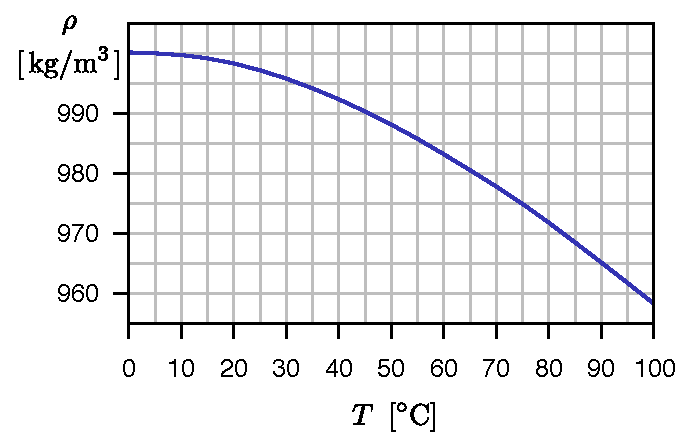
\includegraphics[width=0.8\linewidth]{2014-v3g-03-veeTihedus}
\end{center}

\hint
Ideaalse gaasi olekuvõrrandiga on võimalik määrata, mis õhu ruumalaga avariiventiil avaneks. Õhu ruumala muudust on aga võimalik avaldada vajaliku vee tiheduse muudu.

\solu
Et avariiventiil avaneks, peab rõhk süsteemis kasvama väärtuseni $p=p_0+\Delta p = \SI{2.2}{}p_0$. Paisupaagis olev õhk on seega kokku pressitud ruumalale $V_2=V_1 p_1/p$ (gaasi olekuvõrrandist konstantsel temperatuuril), mis tähendab, et vesi sai paisuda ruumala $\Delta V = V_1-V_2 = \frac{7}{22}V_1$ võrra. See aga moodustab \[\alpha = \frac{\Delta V}{V_0}= \frac{7}{22}\frac{V_1}{V_0}\approx \SI{0.025}{} = \SI{2.5}{}\%\] vee algsest ruumalast. Et vee mass jääb samaks, tähendab see tiheduse kahanemist väärtuseni \[\rho'=\left(\frac{1}{1+\alpha}\right)\rho_0\approx(1-\alpha)\rho_0= \SI{975}{kg/m^3}.\]
Temperatuuri ja tiheduse sõltuvuse graafikult loeme, et see vastab temperatuurile $t_\text{max}=\SI{75}{\degreeCelsius}$.

\probeng{Expansion vessel}
A house’s heating system consists of a big accumulator vessel, in which circulating hot water is kept and an expansion vessel to compensate water’s thermal expansion. The expansion vessel is a vessel with a fixed volume, one part of the vessel is filled with air, the rest is filled with water originating from the heating system that can freely flow back into the system. When all of the water reached the room temperature $t_0=\SI{20}{\degreeCelsius}$, the expansion vessel was filled with compressed air so that the air volume in the vessel was $V_1=\SI{0.080}{m^3}$ and pressure $p_1=\SI{1.5}{}\,p_0$, where $p_0=\SI{0.10}{\mega\pascal}$ is atmosphere pressure. At room temperature the volume of the water in the whole system is $V_0=\SI{1.0}{m^3}$.\\
There is also an emergency valve in the piping to avoid the bursting of the pipes. The valve opens when the pressure in the piping exceeds atmosphere pressure by $\Delta p = \SI{1.2}{} \, p_0 $. To what temperature can the water in the system be heated without there being an accident? Neglect metal’s thermal expansion. The ratio between the density of water and temperature is shown in the graph. Assume that the graph’s shape does not depend on the pressure (the changes in pressures are too small for that). Also assume that the air temperature in the expansion vessel stays at room temperature $t_0$.
\begin{center}
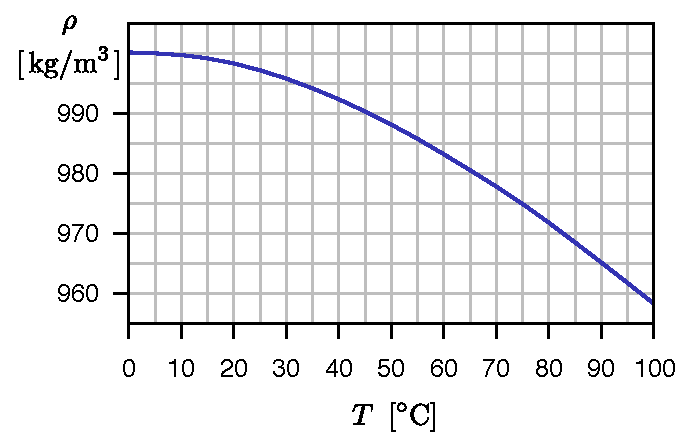
\includegraphics[width=0.8\linewidth]{2014-v3g-03-veeTihedus}
\end{center}

\hinteng
With the ideal gas law it is possible to determine the air volume that is necessary to open the emergency valve. From the change of the air volume it is possible to express necessary change of water density.

\solueng
For the emergency valve to open the pressure in the system has to increase to a value $p=p_0+\Delta p = \SI{2.2}{}p_0$. The air inside the expansion vessel is therefore compressed into a volume $V_2=V_1 p_1/p$ (at constant temperature from the ideal gas law) which means that the water could have expanded by a volume $\Delta V = V_1-V_2 = \frac{7}{22}V_1$. But this forms
\[\alpha = \frac{\Delta V}{V_0}= \frac{7}{22}\frac{V_1}{V_0}\approx \SI{0.025}{} =  \SI{2.5}{}\%\] 
of the initial volume of the water.  Since the mass of the water stays the same it means that the density decreases to a value
\[\rho'=\left(\frac{1}{1+\alpha}\right)\rho_0\approx(1-\alpha)\rho_0= \SI{975}{kg/m^3}.\] 
From the temperature versus density graph we read that it corresponds to the temperature $t_\text{max}=\SI{75}{\degreeCelsius}$.
\probend